\section{Competing Applications}
\label{sec:competition}
With work and school continuing online and many in-person activities still restricted, there can be multiple applications using the home network. Any combination of VCAs, video streaming, or other popular applications may be simultaneously competing for scarce bandwidth. In this section, we measure how VCAs perform in the presence of competing applications. Specifically, we focus on link sharing with other VCAs, TCP flow (iPerf3), and two popular video streaming applications, Netflix and Youtube. 

\begin{comment}
In the ``real world," network links must support multiple applications simultaneously.
How effectively -- or aggressively~-- do VCAs compete with each other applications?
What is the minimum network bandwidth required, to support Meet, Teams, or Zoom 
    in conjunction with each other other common applications?
These questions became critical through the coronavirus pandemic,
  and remain so as remote work remains prevalent.
\end{comment}

    





\begin{figure*}[t]
    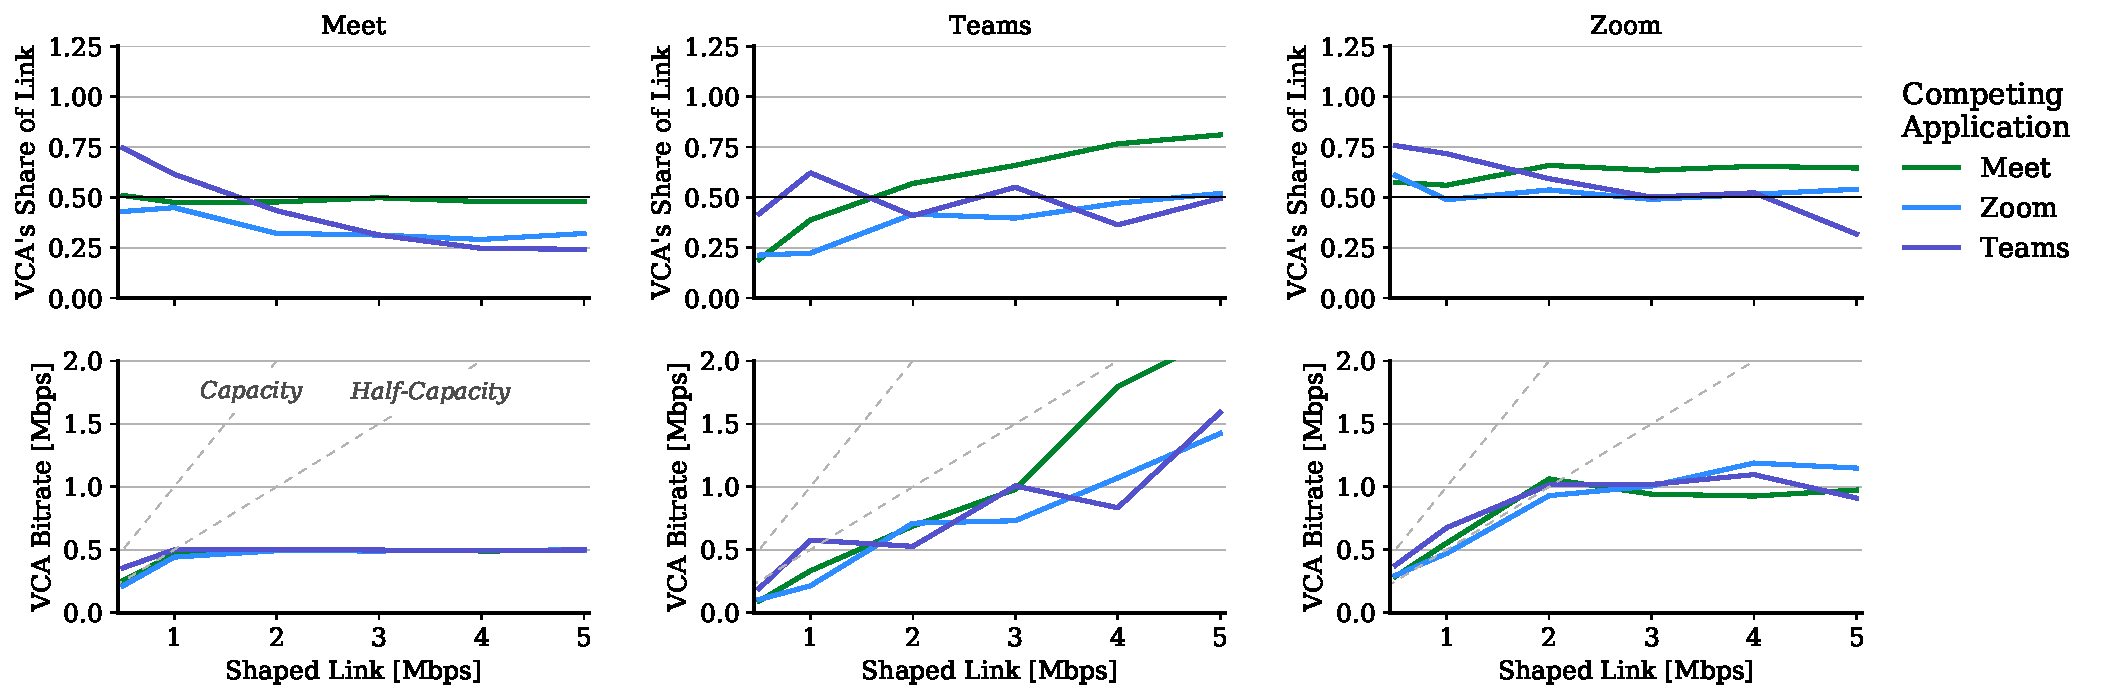
\includegraphics[width=\linewidth]{figures/comp/dl_competition_vca.pdf}
    \caption{Share of downstream link and VCA bitrates for VCAs in competition with other flows, as a function of downlink bitrate cap.}
	\label{fig:comp_bitrates_dl}
\end{figure*}

\begin{figure*}[t!]
\centering
\begin{subfigure}[t]{.33\textwidth}
    \centering
    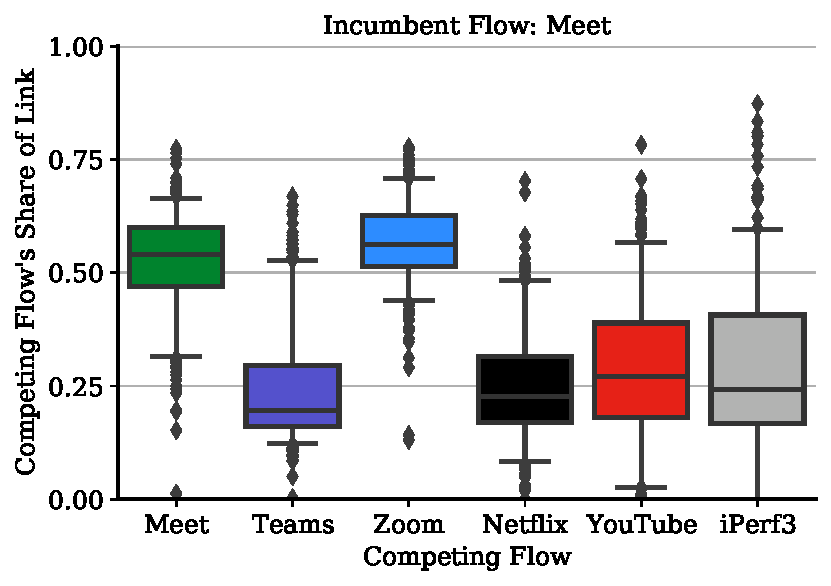
\includegraphics[width=1\textwidth]{figures/comp/box_plot_meet_dl_0.5.pdf}
    \caption{Meet}
    \label{fig:zoom_box_1}
\end{subfigure}\hfill
\begin{subfigure}[t]{.33\textwidth}
    \centering
    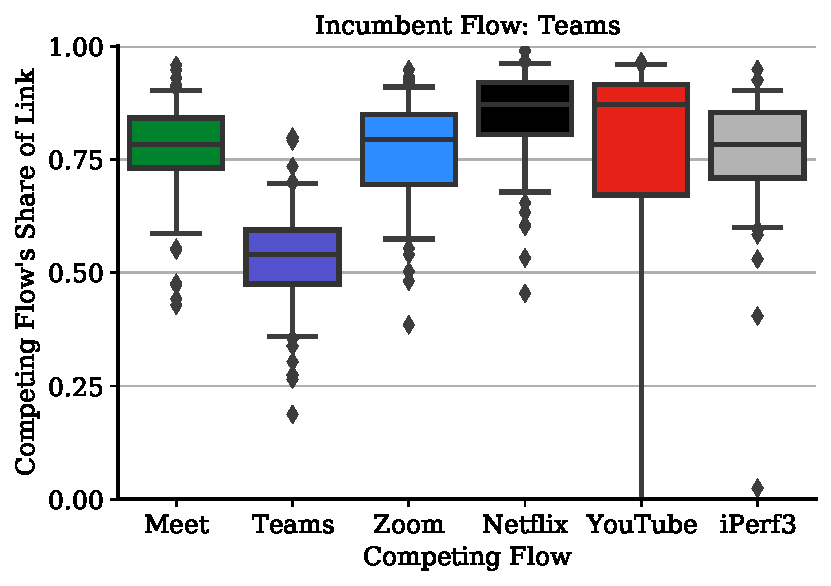
\includegraphics[width=1\textwidth]{figures/comp/box_plot_teams_dl_0.5.pdf}
    \caption{Teams}
    \label{fig:zoom_box_1}
\end{subfigure}
\begin{subfigure}[t]{.33\textwidth}
    \centering
    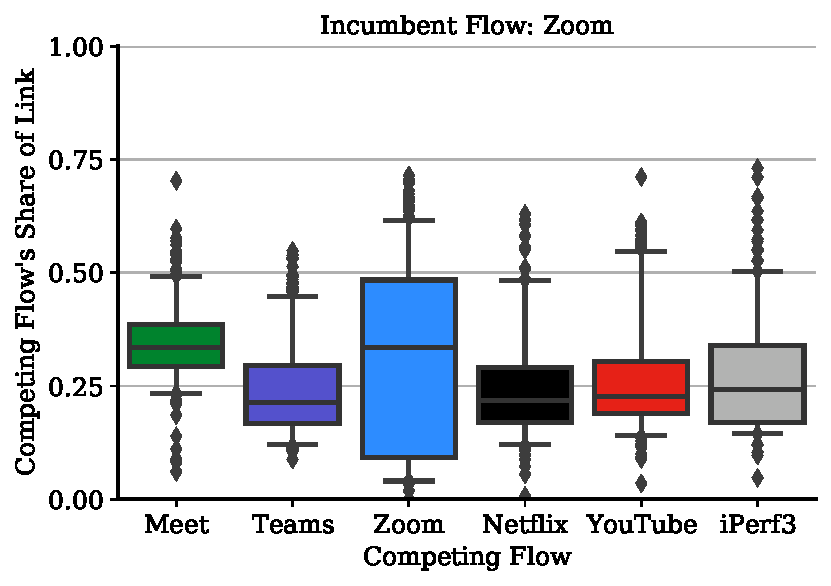
\includegraphics[width=1\textwidth]{figures/comp/box_plot_zoom_dl_0.5.pdf}
    \caption{Zoom}
    \label{fig:zoom_box_1}
\end{subfigure}
\caption{Downstream bitrate of applications in competition with each VCA, with a link shaped symmetrically at 0.5~Mbps.}
\label{fig:dnld-boxplot}
\end{figure*}


\noindent \textbf{Methodology}: As illustrated in Figure \ref{fig:competition-setup}, the setup for these experiments differs slightly from earlier ones. 
Instead of connecting the client directly to the router, the two matched clients, C1 and F1, are connected to the router via a switch. 
The link between the switch and the router is shaped by the router.

For each test, C1 first establishes a VCA call with C2.
Approximately 30 seconds later, F1 establishes a competing flow, which lasts for two minutes.
F1's counter-party, F2, depends on the type of flow.
If the competing flow is another VCA call, then it is another consumer laptop.
If the competing flow is an iPerf3 (TCP) flow, then F2 is a server on the University network
  and if the flow is Netflix or Youtube, then F2 is a server for the respective service.
Netflix and Youtube are launched directly in Chrome via \texttt{xdg-open}.
After the competing flow terminates, the incumbent flow continues for an additional minute.
We repeat each experiment with bandwidth shaped symmetrically at 0.5, 1, 2, 3, 4, and 5~Mbps.

\subsection{Competition with VCAs}

When there are simultaneous VCAs on the same network, there will be competition on both the uplink and downlink. Looking first at the uplink, we observe some differences in how each VCA shares the link. Figure \ref{fig:comp_bitrates_ul} clearly illustrates two operation regions that are defined by each VCA's nominal uplink bitrate. Zoom and Meet reach their nominal bitrate when the link capacity is 2 Mbps. Teams has a significantly higher nominal bitrate than Meet and Zoom, reaching it only once the link capacity is 3 Mbps.

Meet and Teams tend to equitably share the link across all bandwidth capacities while Zoom is aggressive at 0.5 and 1 Mbps capacities. As shown in Figure \ref{fig:boxplot-upld}, Zoom uses around $75\%$ of the available capacity, even when competing against another Zoom call. Interestingly, Teams backs off against the iPerf3 TCP flow, using well under half capacity at all link capacities. 

Turning to downlink sharing, Figure \ref{fig:comp_bitrates_dl} shows how uplink and downlink sharing are not symmetric.%\jamie{Would follow this immediately with examples of how they are not symmetric -- could be Teams saturating earlier on uplink than downlink, or the different, simulcast-generated levels for Meet.}
Immediately noticeable is the consistency at which Meet reaches a stable bitrate.%\jamie{awkward} 
Once the link capacity reaches 1~Mbps, Meet's downlink bitrate does not increase with any further link capacity increases. Similarly, Zoom's downlink bitrate peaks at 1 Mbps, which it reaches once the link capacity is 2 Mbps. However, we observe that Teams is far less efficient in sharing the link with competing VCAs. Teams fails to reach a stable downlink bitrate, even when the link is not saturated. In Figure \ref{fig:comp_bitrates_dl}b, we see that Teams has an average downlink bitrate under 1 Mbps when competing against Zoom on a 3 Mbps link. 

The way each VCA shares the link with other applications is made clear in Figure \ref{fig:dnld-boxplot}. We see that Zoom uses well over $50\%$ of the available capacity against other VCA.


\subsection{Competition with Non-VCAs}
The way each VCA competes with other VCAs is amplified in how they compete with other applications. Meet and Zoom can command over $75\%$ of the available bandwidth against Netflix, Youtube, and iPerf3 while Teams uses under $25\%$. 

\begin{figure}[t]
    \centering
    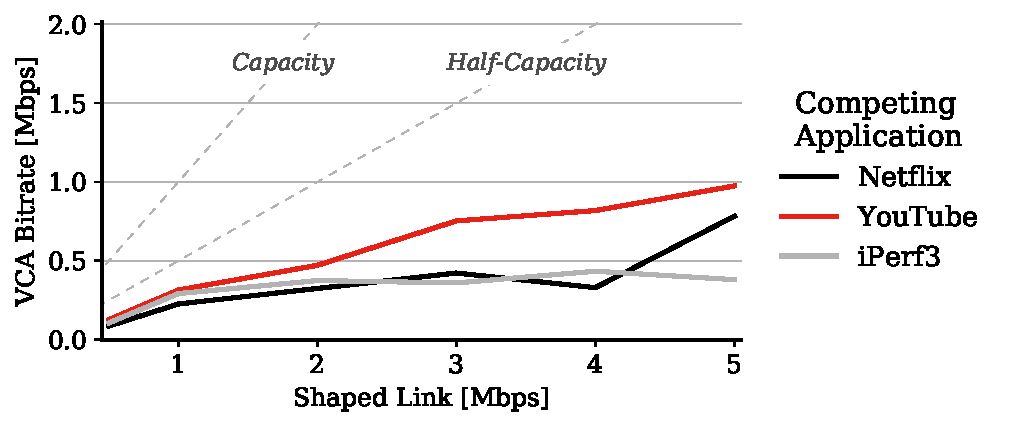
\includegraphics[width=\linewidth]{figures/comp/dl_competition_teams_app.pdf}
    \caption{Share of downstream link and VCA bitrates for VCAs in competition with other flows, as a function of downlink bitrate cap.}
	\label{fig:comp_bitrates_dl}
\end{figure}




\begin{comment}
    \begin{figure}[th]
    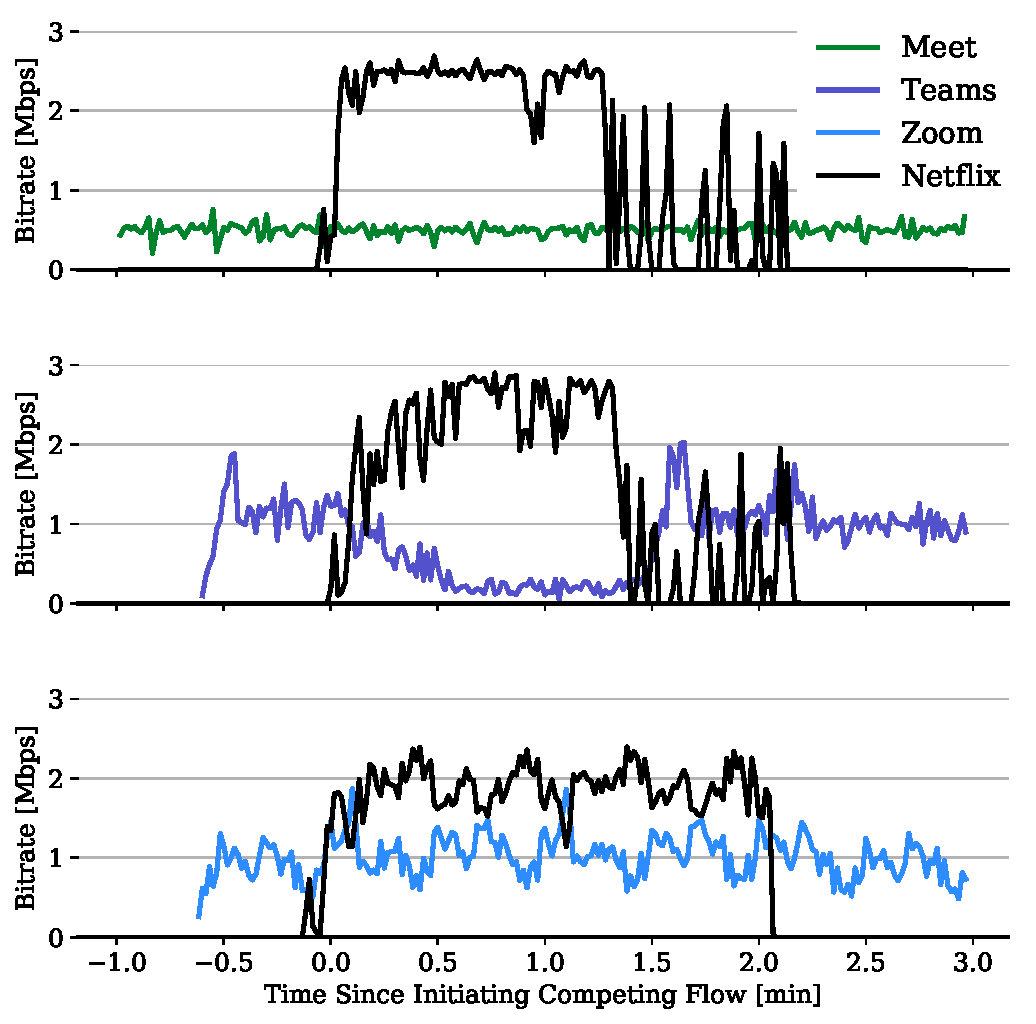
\includegraphics[width=\linewidth]{comp/netflix_time_series.pdf}
    \caption{Teams downlink bitrate when competing against non-VCA applications}
	\label{fig:ts_comp_netflix}
\end{figure}
  
Unlike VCAs, which can not buffer, the average bitrate of video streaming applications can change drastically over time. Figure \ref{fig:ts_zoom_netflix} shows how Netflix and each VCA interact over the course of the experiment. Each interaction is characterized uniquely by a given VCA. \jamie{I would move this up, to part of an `illustration.'}

First, Zoom and Meet do not back off in the presence of Netflix, and continue to receive at the same rate as before. Meet and Zoom both send at a rate lower than $50\%$ of the link capacity. But while Meet and Zoom exhibit similar behavior, their affect on Netflix is different. Because Meet receives at a lower bitrate than Zoom, Netflix maintains a high downlink bitrate as it buffers, before changing to only sporadic bursts of downlink usage. With Zoom, Netflix is not able to buffer, so maintains a constant downlink bitrate. 

Netflix also buffers when competing against Teams. But soon as Netflix is launched, Teams decreases its downlink bitrate, going as low as [insert min bitrate] Mbps. This is both undesirable for VCAs, which are sensitive to changes in bitrate, and an inefficient use of the link. Even in the face of a TCP-based application like Netflix, Teams reduces its downlink consumption. Teams only recovers to its average bitrate once Netflix has finished buffering. 
\end{comment}


% \begin{figure}[t]
%     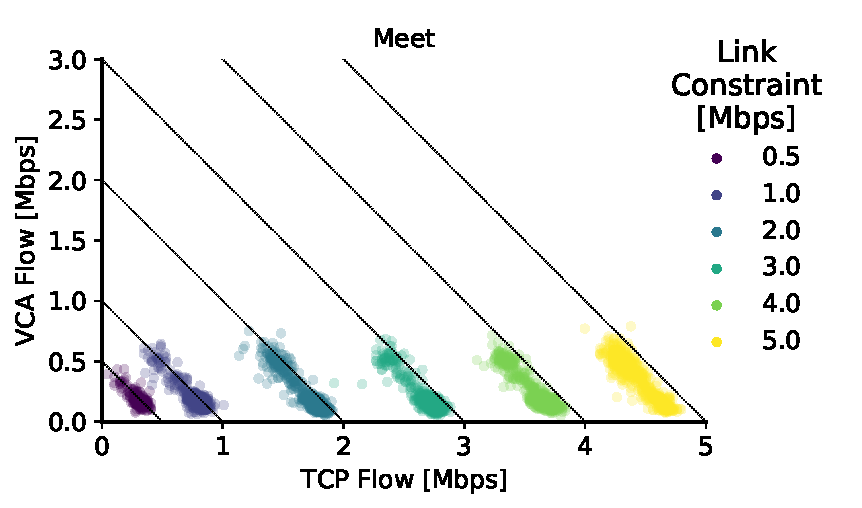
\includegraphics[width=\linewidth]{comp/meet_iperf_scatter.pdf}
%     \caption{Competition between Meet and an iperf3 TCP flow.}
% 	\label{fig:comp_meet_iperf}
% \end{figure}

% \begin{figure}[t]
%     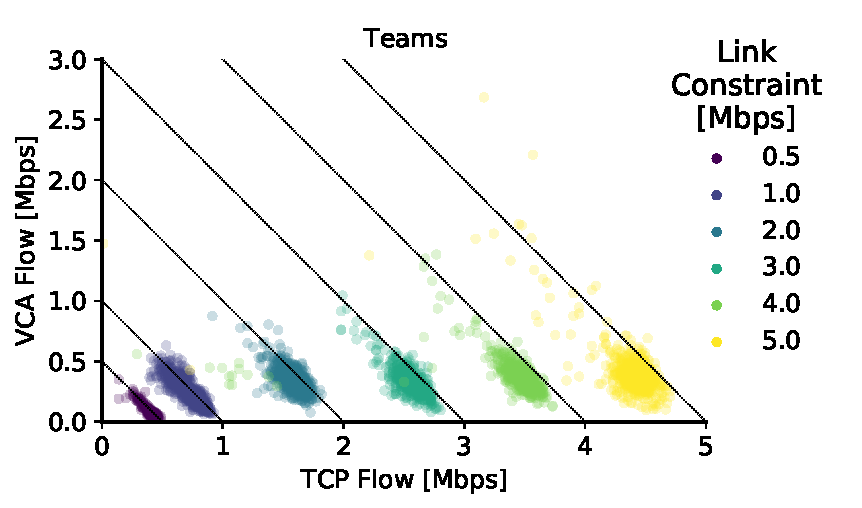
\includegraphics[width=\linewidth]{comp/teams_iperf_scatter.pdf}
%     \caption{Competition between Teams and an iperf3 TCP flow.}
% 	\label{fig:comp_teams_iperf}
% \end{figure}

\begin{comment}
We illustrate the basic setup in Figure~\ref{fig:ts_comp_netflix}, 
  pitting the VCAs against Netflix at on a link constrained to 3~Mbps.

From these flows, we construct two variables
  to reflect fairness and performance in the measured flows.
Fairness is represented 
  as the nominal flow's share of two flows constrained link.
In other words, the denominator for the ``share" is
  is the sum of the two flows rather than 
  the shaped link level.
Performance is proxied by bitrate.
Figure~\ref{fig:comp_bitrates_dl}
  displays results for all three VCAs.


Each application uses half the link in ``competition" with itself.
Competition is in evidence primarily at the low end of the domain,
  with the most severe constraints.
Table~\ref{tab:comp} shows the share
  of the flows that each VCA uses,
  at the most-constrained 0.5~Mbps level.
Here, at the low end, Zoom competes
  aggressively and effectively with all other flows:
  it consumes more than three-quarters of the link against Teams, Netflix, and iperf3, 
  and 0.72 against YouTube.
Meet is also quite aggressive at this level, 
  though Zoom ``wins" in direct competition.
Teams fares worse on very-constrained links,
  and does not even compete with the TCP flow.
  


\begin{table}
    \setlength{\tabcolsep}{3pt}
    \fontsize{10.5}{13} \selectfont
    \centering
\begin{tabular}{lcccccc}
\toprule
{} &       Meet &       Teams &        Zoom &     Netflix &     YouTube & iPerf3 \\
\midrule
Meet  &   \cbss{0.47} &  \cbsss{0.74} &   \cbss{0.43} &  \cbsss{0.76} &  \cbsss{0.71} &  \cbsss{0.72} \\
Teams &    \cbs{0.25} &   \cbss{0.41} &    \cbs{0.23} &     \cb{0.17} &    \cbs{0.26} &    \cbs{0.22} \\
Zoom  &  \cbsss{0.66} &  \cbsss{0.76} &  \cbsss{0.68} &  \cbsss{0.75} &  \cbsss{0.73} &  \cbsss{0.72} \\
\bottomrule
\end{tabular}
    \caption{Share of 0.5 Mbps link. Rows are the ``incumbent" VCAs and columns are competing applications.}
    \label{tab:comp}
\end{table}



With weaker constraints, most applications reach their nominal bitrates
  and the ratios in the upper panels of Figure~\ref{fig:comp_bitrates}
  simply show the ratio of their bandwidth demands.
For example, 
  the low VCA shares with respect to iperf at weak constraint
  simply illustrates the "inexhaustible" demand of a TCP flow,
  whereas link share's of Zoom vs Meet or Meet vs Zoom 
  at link capacity of 5 Mbps (0.4 or 0.6) simply 
  reflect different nominal bandwidths.
As already shown, in the time series plots, there is some subtlety in the timing of competition.
Video streaming services (YouTube and NetFlix)
  can and do buffer, ifthe bandwidth is high enough.
This means that they may not compete most of the time.
The VCAs and the iPerf3 TCP flows on the other hand, 
  are continuous, though only iPerf3 has inexhaustible demand.
The VCAs seem to ``test" the bandwidth early in the call, 
  and the fist moments may not illustrate their long-term strategies.
This is analogous to TCP ``slow-start,"
  but appears to be much slower.

The lower panels of Figure~\ref{fig:comp_bitrates} show
  the VCAs' bitrates, in competition.
Again, Zoom is quick out of the gate, and 
  achieves over 90 of nominal link bitrate,
  for constraints weaker than 2 Mbps.
On the other hand, Teams does not achieve full bitrate
  below 5~Mbps;
  \jamie{at 10~Mbps, it achieves a flow of X}.
Depending on the flow, Meet's used bitrate saturates
  when the shared link has capacity greater than 3 Mbps.
The same is true for Zoom, though its plateau is higher and noisier.
  
\jamie{We start getting repetitive here}
 Looking first at how Meet competes with other VCAs, it uses slightly less than Zoom but dominates Teams. Meet is also remarkably fair when competing with another Meet flow, splitting the available link capacity almost exactly evenly. Against TCP applications, Meet commands roughly $75\%$ of the available link capacity at the 0.5 Mbps shaping level. 

While not quite as consistent as Meet, Zoom nevertheless shares the link in a similar manner regardless of the competing application. At low link capacities, Zoom uses up to [X] \% of the the available bandwidth. By [X] Mbps, its downlink bitrate remainly roughly the same. 

This consistency manifests differently in how Teams competes. 
Where Zoom and Meet aggressively use the available link capacity at low bandwidths, Teams backs off, in almost all cases using less than $25\%$ of the available bandwidth on a 0.5 Mbps downlink connection. Consider first how Teams behaves with other VCAs. While still dominated at the low end, as the link capacity increases and Zoom and Meet reach a stable downlink bitrate, Teams begins to also increase its downlink bitrate. Notice, however, that even at a 5 Mbps link capacity, Teams's downlink bitrate does not exceed 1.25 Mbps. Looking next at how Teams competes with the TCP-based applications, we observe even more startling behavior. When competing against Netflix and the iPerf3 flow, the downlink bitrate never exceeds 0.25 Mbps. This is especially inexpedient given the sensitivity of VCAs to drops in bandwidth and the goal of equitably sharing the link.  \jamie{Maybe careful here?  This isn't necessarily how peaky ``TCP applications" fare, it's how a single continuous flow fares.  It may be that individual TCP requests can get through fine, cf buffer bloat etc.}
\end{comment}
